
\section{Methodology and System Architecture}
Our ADS is implemented in the Unity game engine, integrating neural network inference with the Barracuda engine to support real-time decision-making. The system is designed for both manual and autonomous control, allowing direct comparisons between human and AI-driven behavior.

The Unity-based ADS serves as a testbed for evaluating neural network behavior under controlled conditions. The simulation environment provides real-time feedback on vehicle position, road conditions, and network predictions.


\subsection{Simulation and Interactive Control}
\label{sec:methodologycontrol}
As illustrated in Figure~\ref{fig:simulation_ui}, users can dynamically adjust key simulation parameters, such as:
\begin{itemize}
    \item Motor torque and steering angles.
    \item Neural network inference frequency.
    \item Maximum steering angles
    \item "Time acceleration" for faster evaluation cycles.
\end{itemize}  
The time acceleration mechanism enables rapid execution of simulation scenarios, substantially reducing the duration of robustness evaluations.
\begin{figure}[h]
    \centering
    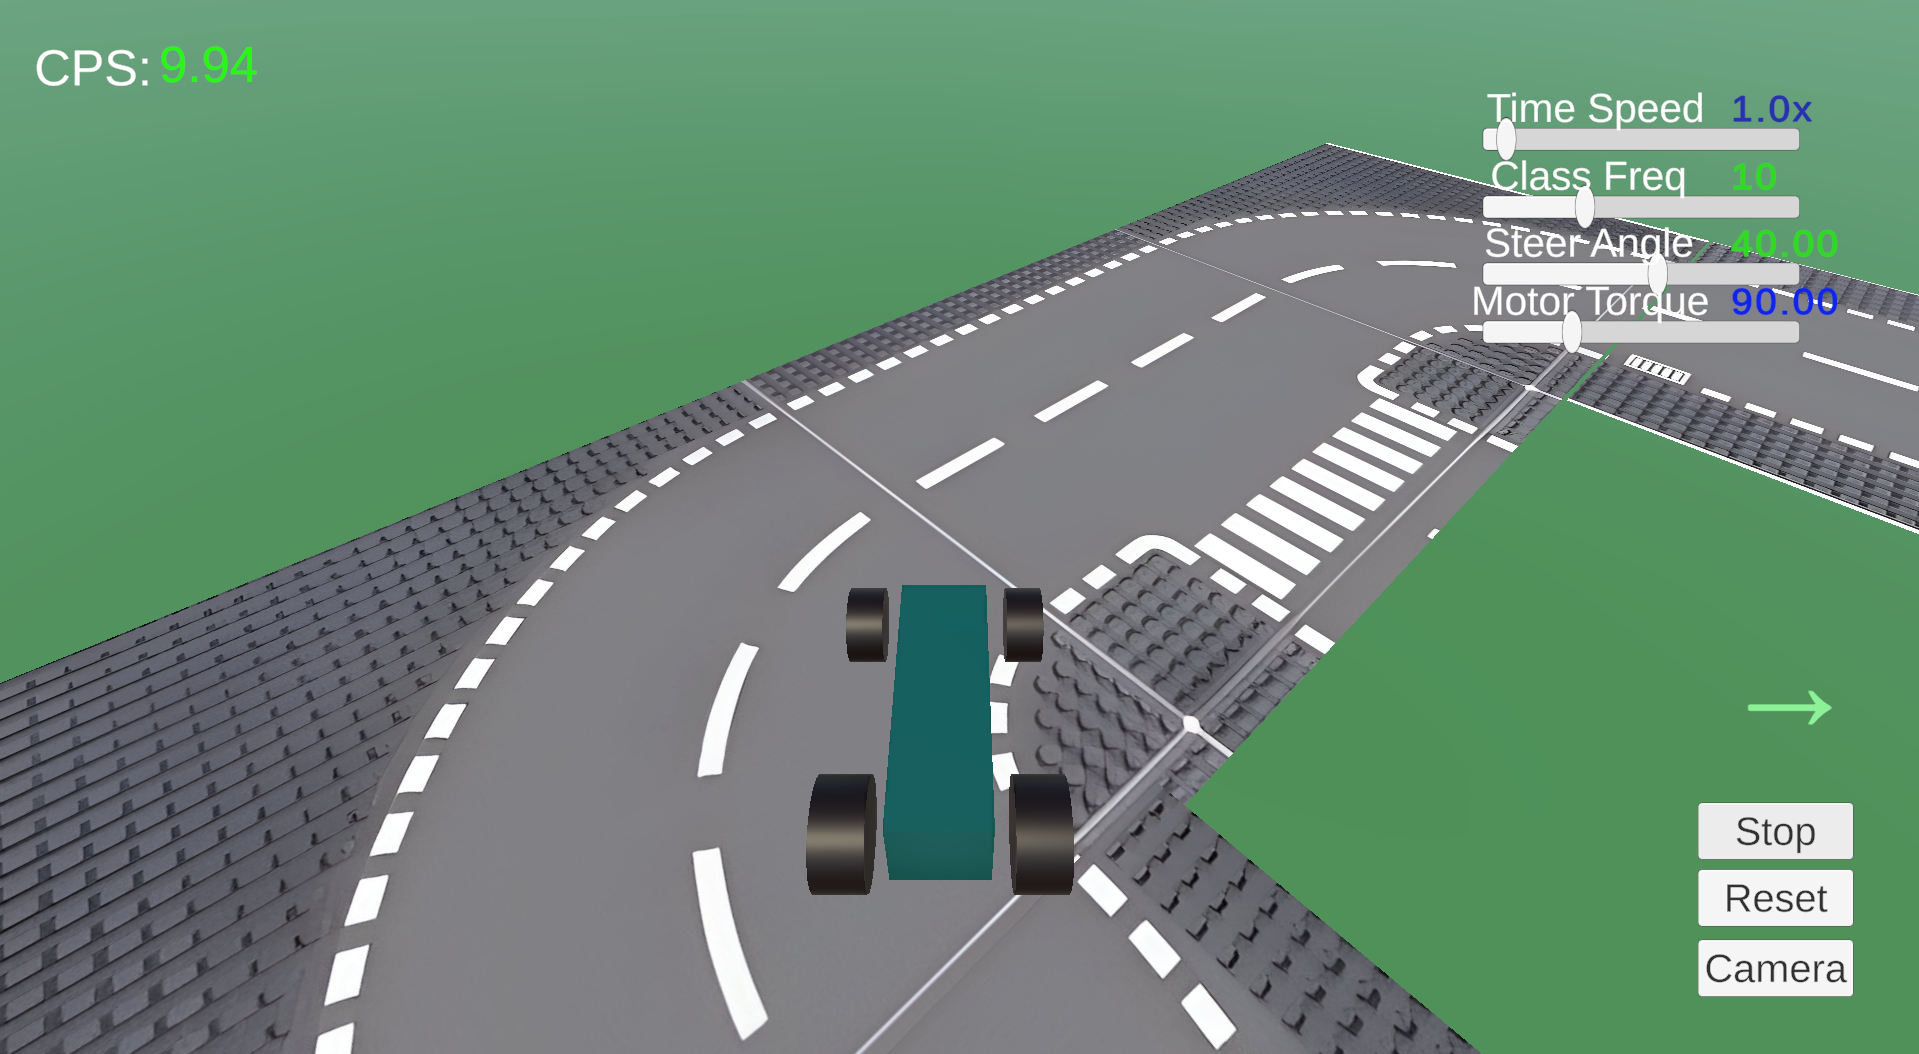
\includegraphics[width=0.9\linewidth]{figures/image.png}
    \caption{Autonomous driving simulation interface with real-time parameter controls for time speed, classification frequency, steering angle, and motor torque. The system displays a runtime classification rate per second (CPS). A green directional arrow visualizes the neural network's predicted driving action. Interactive controls (Stop, Reset, Camera) are provided for simulation management.}

    \label{fig:simulation_ui}
  \end{figure}



 

\subsection{Data Collection and Curation}
\label{sec:data_collection}

As part of our prototype development workflow, we constructed a custom dataset specifically tailored for training and evaluating our vision-based autonomous driving system. The dataset was captured entirely within the 3D driving simulator described in Section~\ref{sec:methodologycontrol}, built using the Unity game engine. To offer visual insight into the collected data, Figure~\ref{fig:dataset-samples} presents a selection of raw RGB images representing the three action classes: \texttt{Forward}, \texttt{Left}, and \texttt{Right}. These samples reflect the diversity of driving conditions captured through the system's forward-facing camera and highlight the visual structure leveraged during training.
 \begin{figure}[h]
 \centering
 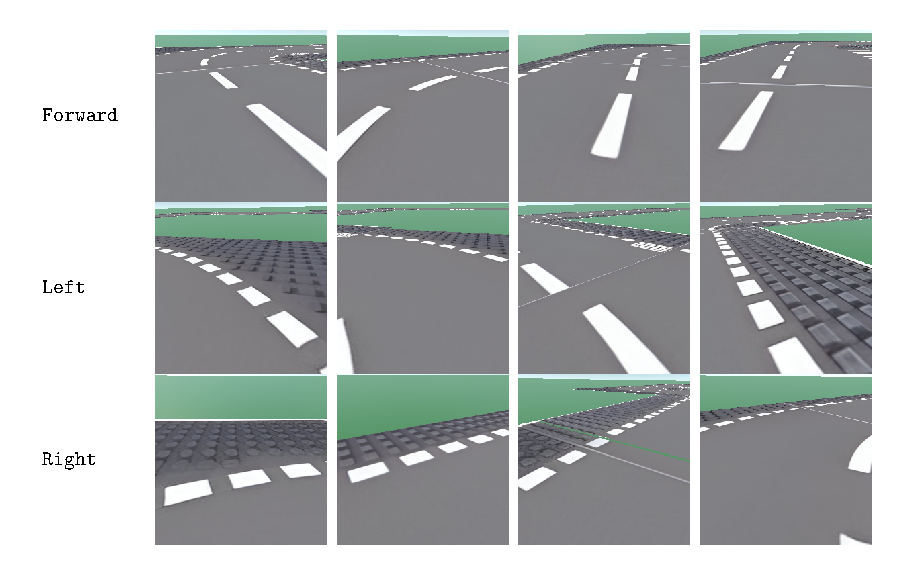
\includegraphics[width=0.95\linewidth]{figures/samples.pdf}
 \caption{Example RGB image samples from the custom dataset, grouped by their corresponding action labels.}
 \label{fig:dataset-samples}
 \end{figure}
\subsubsection{Initial Data Acquisition}
Initial data acquisition was conducted via manual teleoperation of the vehicle. A human operator navigated the track using keyboard inputs corresponding to three discrete actions: \texttt{Forward}, \texttt{Left}, and \texttt{Right}. To generate a labeled sample, the operator triggered a capture command that saved a single data point. Each sample consists of a raw 256$\times$256 pixel RGB image captured from the vehicle's forward-facing camera and its corresponding action label. This initial phase yielded a raw dataset of  2,516 samples.

\subsubsection{Data Preprocessing and Labeling Strategy}
Prior to training, each captured RGB image underwent a standardized preprocessing pipeline to align with the input requirements of our CNN architecture. The pipeline consists of two steps:
\begin{enumerate}
    \item Conversion from RGB to a single-channel grayscale representation.
    \item Down-sampling of the image resolution to 28$\times$28 pixels.
\end{enumerate}

Some driving scenarios can be inherently ambiguous—even for humans. For instance, the second sample in the \texttt{Forward} row or the third sample in the \texttt{Left} row of Figure~\ref{fig:dataset-samples} could plausibly be interpreted as either continuing straight or initiating a turn. While such frames may seem intuitive to a human driver, they can introduce uncertainty for a learning-based system. A core tenet of our data curation was to mitigate this kind of label ambiguity, which can inhibit effective model training. To this end, a strict labeling heuristic was adopted: \texttt{Left} and \texttt{Right} labels were applied exclusively to frames captured as the vehicle was actively approaching or navigating corners or edges of the track. All other frames depicting uninterrupted, forward-aligned driving were labeled as \texttt{Forward}. This strategy proved critical for achieving robust driving performance, as it provides the model with clear, context-dependent training signals.

\subsubsection{Model-in-the-Loop Refinement}
To further enhance dataset quality, we employed a model-in-the-loop refinement cycle. The curated dataset was partitioned into a training set (88.97\%) and a test set (11.03\%) using a stratified, temporally ordered split. Samples were first grouped by class, then chronologically sorted within each group to preserve their temporal structure. The most recent 11.03\% of each class was assigned to the test set, ensuring class balance while minimizing temporal leakage. A baseline CNN was trained on the resulting training set and deployed via the Barracuda inference engine within the Unity environment. To assess its real-world viability, the trained model was tasked with autonomously completing three consecutive laps of the track without deviating off course.

In instances of failure, the specific track region causing the error was identified. A targeted data collection session was then initiated to gather additional, focused samples from this problematic area. These new samples were integrated into the primary dataset, and the refinement cycle of cleaning, splitting, training, and real-time evaluation was repeated.

\subsubsection{Final Dataset Characteristics}
The iterative refinement process concluded once the baseline model could consistently achieve the two-lap objective. The final, curated dataset used for all experiments in this study comprises \textbf{1,814} high-quality samples. The final class distribution is detailed in Table~\ref{tab:dataset_dist}. The distribution, with a preponderance of \texttt{Forward} samples, reflects the natural driving behavior on a looped track, which involves more time spent driving straight than turning. This meticulously prepared dataset serves as the definitive basis for training and robustly evaluating the models explored in this study.

\begin{table}[h!]
\centering
\caption{Final distribution of samples in the curated dataset.}
\label{tab:dataset_dist}
\begin{tabular}{@{}lcc@{}}
\toprule
\textbf{Class Label} & \textbf{Sample Count} & \textbf{Percentage} \\ \midrule
Forward              & 750                   & 41.3\%              \\
Right                & 522                   & 28.8\%              \\
Left                 & 542                   & 29.9\%              \\ \midrule
\textbf{Total}       & \textbf{1,814}        & \textbf{100.0\%}    \\ \bottomrule
\end{tabular}
\end{table}





%
 \begin{figure}[h]
 \centering
 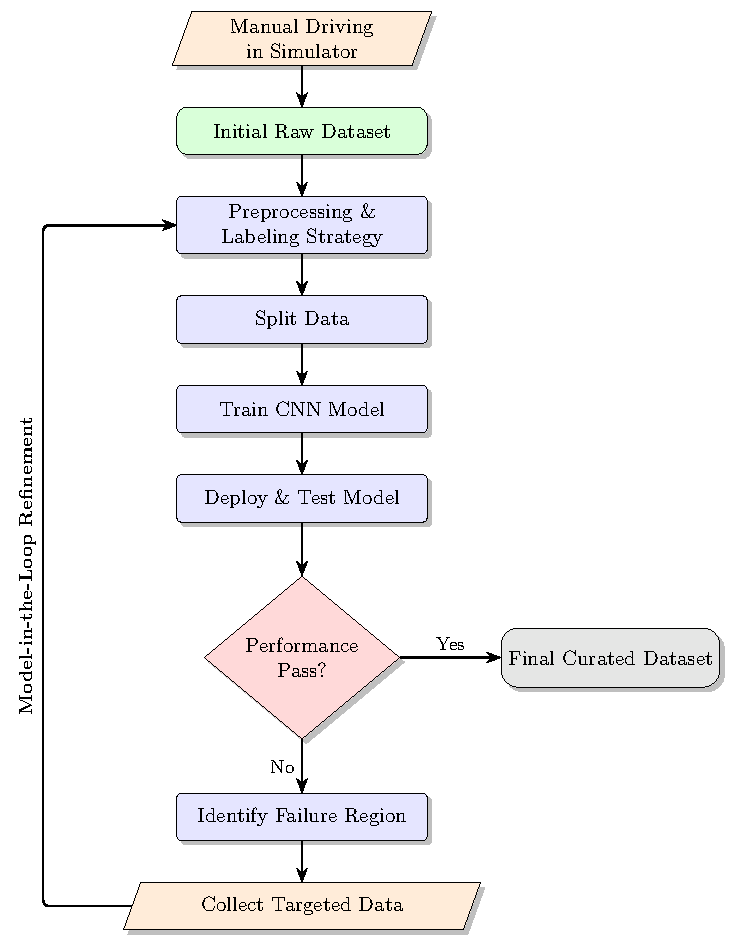
\includegraphics[width=0.8\linewidth]{figures/flow_chart.pdf}
 \caption{The iterative data collection and model-in-the-loop refinement process. The cycle begins with manual data acquisition and proceeds through training and evaluation. If the model fails the performance test, targeted data is collected from failure regions and integrated back into the dataset, repeating the cycle until the performance objective is met.}
 \label{fig:simulator}
 \end{figure}

\subsection{Neural Network Architectures}
\label{sec:nn-architectures}

To systematically study the trade-off between network size and verifiability, we constructed a family of convolutional neural network (CNN) models designed specifically for image classification tasks with grayscale inputs of size $28 \times 28$ pixels. Each model outputs one of three possible classes.

All networks share a consistent two-layer convolutional architecture followed by a compact fully connected head, as illustrated in Figure~\ref{fig:cnn-arch}. The convolutional layers employ $3 \times 3$ kernels, a stride of 2, and padding of 1, sequentially reducing the spatial dimensions from $28 \times 28$ to $7 \times 7$. The output of the convolutional backbone is flattened and passed through a fully connected layer with a fixed hidden size of 4, or 3 in the case of Model~239, before the final classification layer producing 3 output logits.



\begin{figure}[ht]
\centering
\begin{tikzpicture}
    \node at (0,0) {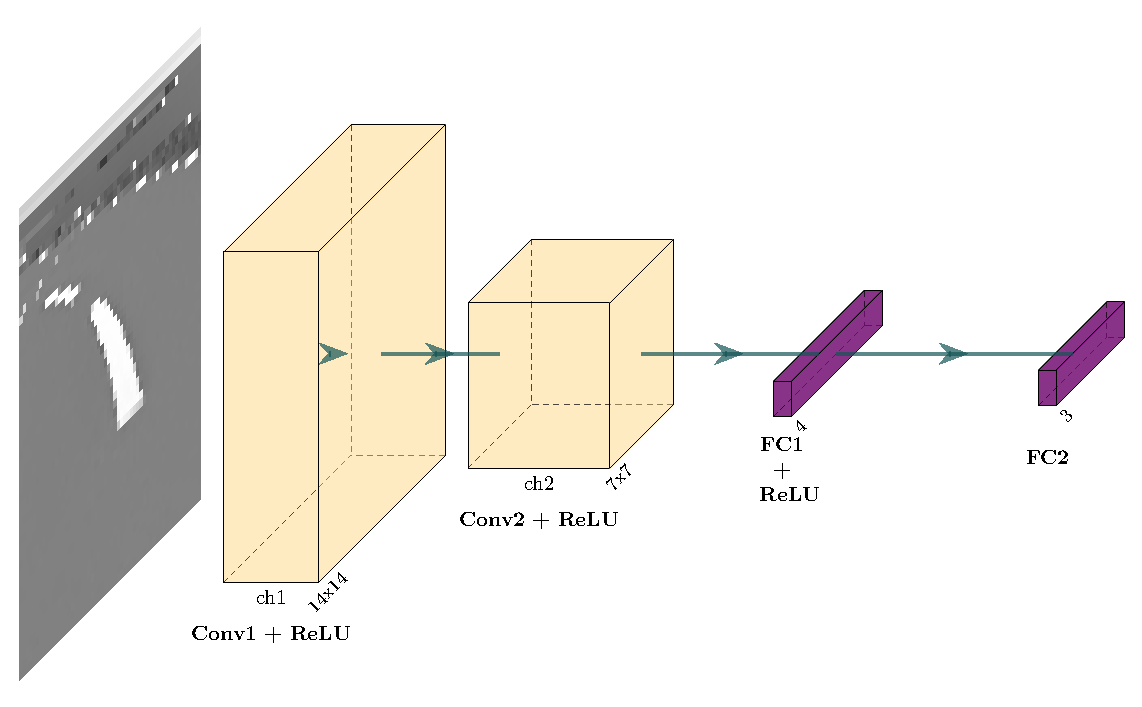
\includegraphics[width=\textwidth]{figures/test_simple.pdf}};

\end{tikzpicture}
\caption{The common CNN architecture used for all models. It consists of two convolutional layers followed by two fully connected layers. The number of channels in the convolutional layers ($ch_1, ch_2$) varies across models as detailed in Table~\ref{tab:model-params}.}
\label{fig:cnn-arch}
\end{figure}

The specific hyperparameter configurations for the different model sizes used in our study are detailed in Table~\ref{tab:model-params}.

\begin{table}[htbp]
\centering
\caption{Model parameter configurations. The number of channels in the first ($ch_1$) and second ($ch_2$) convolutional layers are varied to achieve different total parameter counts.}
\label{tab:model-params}
\begin{tabular}{l c c r}
\toprule
\textbf{Model} & \textbf{$ch_1$} & \textbf{$ch_2$} & \textbf{Total Parameters} \\
\midrule
239    & 4  & 1  & 239 \\
1k    & 4  & 4  & 991 \\
5k  & 10 & 17  & 4,998 \\
20k   & 37 & 37 & 19,999 \\
\bottomrule
\end{tabular}
\end{table}



\subsection{Verification Approach}\label{sec:verificationApproach}

  To formally evaluate the robustness and reliability of neural network predictions, we employ state-of-the-art verification tools including \(\alpha,\beta\)-CROWN and Marabou. These tools enable rigorous assessment of the neural network's resilience to input perturbations, ensuring that minor variations in sensor data do not produce unsafe or unpredictable outcomes. Integrating such verification processes directly into our system's evaluation pipeline enhances confidence in deploying neural network controllers in safety-critical scenarios.


\subsection{Formal Verification Properties}
\label{sec:formal-properties}

Consider a labelled sample \((\boldsymbol{\hat{x}},y)\) drawn from the dataset, where
\(y\in\{1,\ldots,C\}\) is the ground-truth class.  
The network under verification is a mapping
\[
  \mathcal{N} : \mathbb{R}^{n} \longrightarrow \mathbb{R}^{C},\qquad
  \boldsymbol{\hat{x}}\mapsto
  \mathcal{N}(\boldsymbol{\hat{x}})
  =\bigl(\mathcal{N}(\boldsymbol{\hat{x}})_{1},\dots,\mathcal{N}(\boldsymbol{\hat{x}})_{C}\bigr).
\]
We call \(\mathcal{N}(\boldsymbol{\hat{x}})\) the \emph{nominal output vector}.
For a perturbation budget \(\varepsilon>0\) define the $\ell_{\infty}$-ball
\[
  \mathbb{B}_{\infty}(\boldsymbol{\hat{x}};\varepsilon)
  \;=\;
  \bigl\{\boldsymbol{x}\in\mathbb{R}^{n}\mid
        \|\boldsymbol{x}-\boldsymbol{\hat{x}}\|_{\infty}\le\varepsilon\bigr\}.
\]
We term its elements \(\boldsymbol{x}\) \emph{perturbed inputs}, and their corresponding outputs \(\mathcal{N}(\boldsymbol{x})\) are the \emph{perturbed output vectors}.
The formal properties below reference the ground-truth label \(y\).

Following Casadio et al.~\cite{casadio2022neural} we employ three canonical
robustness properties:

\begin{itemize}
%---------------------------------------------------------------
\item \textbf{Classification Robustness (CR).}
      The network must assign the correct class to every input in the
      perturbation set:
      \[
        \forall\,\boldsymbol{x}\in\mathbb{B}_{\infty}(\boldsymbol{\hat{x}};\varepsilon):\quad
        \arg\max_{i}\mathcal{N}(\boldsymbol{x})_{i}=y.
      \]
%---------------------------------------------------------------
\item \textbf{Standard Robustness (SR).}
      For a tolerance \(\delta>0\) the maximal coordinate change in the logit
      vector is bounded by \(\delta\):
      \[
        \forall\,\boldsymbol{x}\in\mathbb{B}_{\infty}(\boldsymbol{\hat{x}};\varepsilon):\quad
        \|\mathcal{N}(\boldsymbol{x})-\mathcal{N}(\boldsymbol{\hat{x}})\|_{\infty}\le\delta.
      \]
%---------------------------------------------------------------
\item \textbf{Strong Classification Robustness (SCR).}
      For a confidence floor \(\eta>0\) the logit of the correct class never
      falls below \(\eta\):
      \[
        \forall\,\boldsymbol{x}\in\mathbb{B}_{\infty}(\boldsymbol{\hat{x}};\varepsilon):\quad
        \mathcal{N}(\boldsymbol{x})_{y}\ge\eta.
      \]
\end{itemize}


These three definitions form the formal foundation of our verification setup. Section~\ref{sec:task-adaptation} explains how we adapt \(\delta\) and \(\eta\) to better fit the task, while Section~\ref{sec:results} presents the specific values used for all hyper-parameters, including \(\varepsilon\).
  